\FloatBarrier

\begin{figure}[h!]
	\centering
	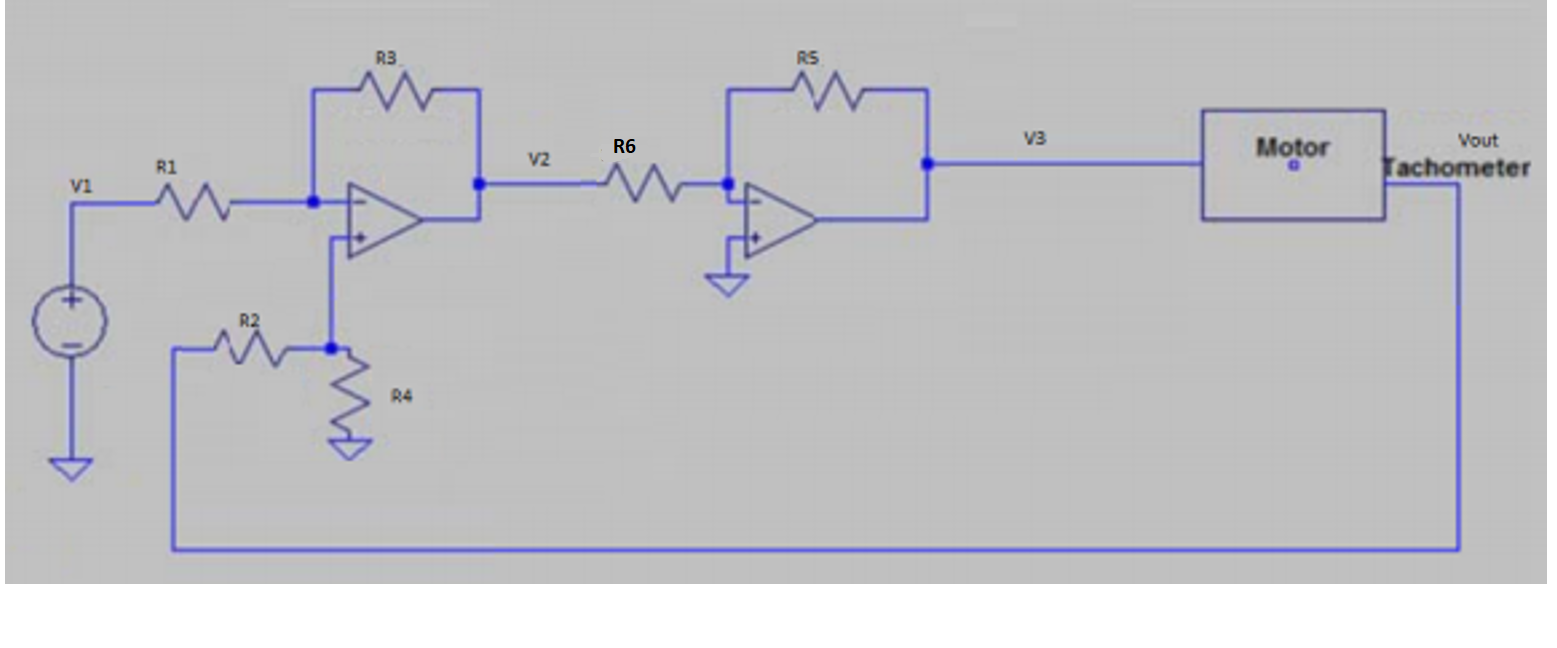
\includegraphics[scale=0.75]{../images/schem6.PNG}
	\caption{Feedback Control System Circuit}
	\label{fig:schem6}
\end{figure}

\FloatBarrier
The first amplifier is a voltage subtractor.
The transfer function for the voltage subtractor in the circuit is given by equation (\ref{eq:tf_sub}).

\begin{equation}
	\label{eq:tf_sub}
	V_{out}(s) = -\frac{ R_3 }{ R_1 }V_{in}(s) + \frac{ R_4 }{ R_2 + R_4 } \frac{ R_1 + R_3 }{ R_1 } V_{out}(s)
\end{equation}

The feedback gain is $0.4$.
So, the input to the feedforward gain is $V_{in} - 0.4V_{out}$.
The feedforward gain is $4$ and is implemented using an inverting amplifier.
The inverting amplifier provides a gain of $-4$.
Therefore, the subtractor must provide an output of $-V_{in} + 0.4V_{out}$ to ensure the proper input is provided to the DC machine.

By equation (\ref{eq:tf_sub}), $\frac{R_3}{R_1} = 1$.
Therefore, $R_3 = R_1$.
If $R_1$ is provided, $R_3$ is determined to have the same resistance.

Substitute $R_3 = R_1$ into equation (\ref{eq:tf_sub}) and consider $V_{out}(s)$'s coefficient.

\begin{equation}
	\label{eq:solve_for_r2r4}
	\frac{2 R_4}{R_2 + R_4} = \frac{1}{2}
	\rightarrow 2 R_4 = \frac{R_2 + R_4}{2}
	\rightarrow \frac{3}{2} R_4 = \frac{R_2}{2}
	\rightarrow R_2 = 3 R_4
\end{equation}

Therefore, if $R_4$ is provided, then $R_2$ is determined to have thrice the resistance.

The inverting amplifier's gain is $-4$ and also given by $-\frac{R_5}{R_6}$.
Therefore, $R_5 = 4 R_6$.
If $R_6$ is provided, $R_5$ is determined to be $4 R_6$.

The following ratios must hold in the circuit.
Assume that $R_1$, $R_4$, and $R_6$ are free parameters.
$R_3$ could also be a free parameter instead of $R_1$, $R_2$ instead of $R_4$, or $R_5$ instead of $R_6$.

\begin{equation}
	\label{eq:final_r3_r1}
	R_3 = R_1
\end{equation}

\begin{equation}
	\label{eq:final_r2_r4}
	R_2 = 3 R_4
\end{equation}

\begin{equation}
	\label{eq:final_r5_r6}
	R_5 = 4 R_6
\end{equation}
